\documentclass[12pt,openany,oneside]{book}
%
\usepackage[utf8]{inputenc}
\usepackage[T1]{fontenc}
\usepackage{lmodern}
\usepackage[english]{babel}
\newcommand{\og}{«\:}
\newcommand{\fg}{»\:}
%
\usepackage{amsmath}
\usepackage{amssymb}
\usepackage{amsfonts}
\usepackage{amsthm}
%
\usepackage{algorithm}
\usepackage{algpseudocode} % For algorithmic environment
%
\usepackage{cite}
\usepackage{hyperref}
%
\usepackage{graphicx}
\usepackage{svg}
%
\usepackage{subcaption}
%
% \usepackage{parskip}
\usepackage{indentfirst}
%
\usepackage{pgfplots}
\pgfplotsset{compat=1.15}
\usetikzlibrary{patterns}
\usepackage{mathrsfs}
%
\usepackage[most]{tcolorbox}
%
\newtcolorbox{problem}[1][]{
  enhanced,
  attach boxed title to top left={yshift=-3mm, yshifttext=-1mm, xshift=0.05\textwidth},
  colback=white,         % default background (white for most document classes)
  colframe=black,        % black frame
  colbacktitle=white,    % white background for title area
  coltitle=black,        % black text in title
  fonttitle=\bfseries,   % bold title font
  after skip=1em,
  title=#1
}
%
\usepackage{geometry}
\newgeometry{top=1.5in,bottom=1.5in,left=1.2in,right=1.2in}
%
\usepackage{fancyhdr} % MUST BE AFTER LOADING GEOMETRY AND GEOMETRY SETTINGS !!
\setlength{\headheight}{30pt}
\pagestyle{plain}
%
\renewcommand{\chaptermark}[1]{\markboth{\chaptername\ \thechapter.\ #1}{}} % This actually sets \leftmark
\renewcommand{\sectionmark}[1]{\markright{\thesection.\ #1}} % This sets \rightmark
%
\fancyhead[L]{\nouppercase{\leftmark} \\
             \hfill \nouppercase{\rightmark}
}
\fancyhead[R]{}
%
\newenvironment{examples}{\textbf{Examples.}\begin{itemize}}{\end{itemize}}
%
\theoremstyle{definition}
\newtheorem{definition}{Definition}
\newtheorem{theorem}{Theorem}
\newtheorem{corollary}{Corollary}
\newtheorem{notation}{Notation}
\newtheorem{proposition}{Proposition}
\newtheorem{remark}{Remark}
\newtheorem{hypothesis}{Hypothesis}
\newtheorem{example}{Example}
%
\numberwithin{definition}{section}
\numberwithin{theorem}{section}
\numberwithin{corollary}{section}
\numberwithin{proposition}{section}
\numberwithin{notation}{section}
\numberwithin{remark}{section}
\numberwithin{hypothesis}{section}
\numberwithin{example}{section}
%
\renewcommand\thesubsubsection{\thesubsection.\alph{subsubsection})}
\setcounter{secnumdepth}{3}
\setcounter{tocdepth}{3}
%
\title{\textbf{Optimization and beyond}}
\author{William DRIOT}
\date{2025-2026}
%
% Conventions for this book :
% 1. Environments should be written this way
%   \begin{...}
%       ...
%   \end{...}
% 2. The terms defined in a definition should be in italics.
% 3. Definition should have names : \begin{definition}[Deterministic Turing machine] ... \end{definition}
% 4. Definition names should use singular names.
% 5. We should comply with the rule that says that equations should be accordingly punctuated : 
%   \[
%     \forall x \in E, ... ,
%   \]
%   or
%   \[
%     \forall x \in E, ... .
%   \]
\begin{document}

\maketitle

\tableofcontents

\setlength{\parindent}{15pt}
\setlength{\parskip}{6pt}

\newpage

\chapter*{Introduction}
\pagestyle{fancy}

Throughout the years, I have learnt to learn. 

One of the strongest conclusion that I came up to is that the best way (for me) to learn, is to write down things that I have understood, clearly, with my words, in the way that I have done here in this document. This enables good understanding, memorizing, and to ensure thorough study of the state of the art, whatever topic I am deep diving into.

Besides ensuring a great understanding of notions, this document also provides proof to anyone as to how determined, passionate and committed I can be.

During this gap year, I have, although not as much as theoretically possible, more time than ever to perform such deep and thorough diving. Last year, R. A. Dragomir and  O. Fercoq's lectures on optimization made me go nuts, and I have likely decided that this branch of mathematics will be the one I ought to dedicate my life to.

I am excited to start my journey by building the strong foundations laid out in this document

\textit{Vivent les mathématiques !}

% I have studied cont. opt., comb. opt. ; 

\part{Continuous optimization}

\chapter{Linear optimization}

\section{The problem}
The references for this chapter include \cite{hurlbert2009}, \cite{dantzig1997}, \cite{dantzig2002}, \cite{chvatal1983}, as well as \cite{karmarkar1984}.

Usual introductions to the simplex algorithm start the following way : consider a company that has $ n $ products to sell. It shall produce nonnegative (not necessarily integral) amounts $ x_1,...,x_n $ of each product. To do so, the company makes use of $ m $ machines, each can respectively run $ b_1, ..., b_m $ minutes per month. Each product must pass though each machine, during an amount proportional to the quantity that must be produced : for each $ 1 \le j \le n $ and each $ 1 \le i \le m $, producing an amount $ x_j $ of the $ j $-th product requires machine $ i $ to run $ a_{ij}x_j $ minutes. So, the amounts $ x_j $ must satisfy the contraints
\[
    \forall i \in \{ 1,...,m \}, \sum_{j=1}^n a_{ij} x_j \leqslant b_i.
\]
Recall that the produced amounts can only be nonnegative, so we must also have
\[
    \forall j \in \{ 1,...,n \}, x_j \geqslant 0.
\]
Finally, the $ j $-th product will be sold at cost $ c_j $. The company then wants to maximize its profit
\[
    \sum_{j=1}^n c_j x_j.
\]
The motivates the Simplex problem.

\begin{problem}[Linear optimization problem]
    \textbf{Given} real numbers $ (a_{ij})_{\substack{1 \leq i \leq m \\ 1 \leq j \leq n}} $, $ (b_j)_{1 \leq j \leq n} $, $ (c_i)_{1 \leq i \leq m} $,

    \textbf{Maximize} over the real numbers $ x_1, ..., x_n $, the quantity
    \[
        \sum_{i=1}^n c_i x_i,
    \]

    \textbf{Under the constraints}
    \[
        \forall i \in \{ 1, ..., m \}, \sum_{j=1}^n a_{ij} x_j \leqslant b_i,
    \]
    \[
        \forall j \in \{ 1, ..., m \}, x_j \geqslant 0.
    \]
\end{problem}

This problem can be reformulated in its (obviously equivalent) matrix form

\begin{problem}[Linear optimization problem]
    \textbf{Given} a matrix $ A \in \mathbf R^{m \times n} $ and vectors $ b \in \mathbf R^m $, $ c \in \mathbf R^n $,

    \textbf{Maximize} over the vector $ x \in \mathbf R^n $, the linear form
    \[
        c^\top x,
    \]

    \textbf{Under the constraints}
    \[
        Ax \leqslant b,
    \]
    \[
        x \geqslant 0.
    \]
\end{problem}

Here, we have used the notation $ x \leqslant y $ to denote the condition $ x_i \leqslant y_i $ for all $ i \in \{ 1, ..., d \} $.

\begin{example}
    For instance, assume we want to maximize the linear form
    \[
        z = 400x + 200y
    \]
    under the constraints
    \[
        \left\{
        \begin{array}{ccc}
            30x + 20y \leqslant 6000 \\
            40x + 10y \leqslant 4000 
            x,y \geqslant 0
        \end{array}
        \right.
    \]
    Then, the problem can be represented as in the following drawing :

    \begin{center}
        \begin{tikzpicture}[x=0.03cm,y=0.015cm]
            \fill[yellow!50] (0,0) -- (100,0) -- (40,240) -- (0,300) -- cycle;

            % Axes
            \draw[->] (-5,0) -- (220,0) node[below right] {$x$};
            \draw[->] (0,-5) -- (0,420) node[above left] {$y$};

            \foreach \x/\lab in {40/40,100/100,200/200}{
            \draw (\x,0) -- (\x,-5) node[below] {\lab};
            }

            \foreach \y/\lab in {200/200,240/240,400/400}{
            \draw (0,\y) -- (-5,\y) node[left] {\lab};
            }

            \draw[thick] (0,400) -- (100,0)
            node[pos=0.42,above left,sloped] {$40\,x + 10\,y = 4000$};

            \draw[thick] (0,300) -- (200,0)
            node[pos=0.65,above,sloped] {$30\,x + 20\,y = 6000$};

            \draw[thick,red,yshift=-10,xshift=-10] (0,300) -- (150,0)
            node[pos=0.75,above,sloped] {$400\,x + 200\,y = \lambda$};

            \fill (40,240) circle [radius=1.2];
            \draw[densely dotted] (40,0) -- (40,240);
            \draw[densely dotted] (0,240) -- (40,240);
        \end{tikzpicture}
    \end{center}

    The family of lines
    \[
        D_\lambda = \{ (x,y) \in \mathbf R^2, 400x + 200y = \lambda \}
    \]
    is a family of parallel lines. The problem is to find the maximum value of $ \lambda $ such that $ D_\lambda $ meets the regions of constraints.
\end{example}

Looking at the figure, it appears clear that the maximum is attained at the point of coordinates $ (40,240) $ which has been highlighted for that reason. The development of the Simplex algorithm establishes the following fact which applies to all situations.

\begin{theorem}
    If a linear optimization problem admits a solution, its optimal solution(s) exists and is(are) attained on a an extremal point of the constraints region.
\end{theorem}

On a side note, recall that :

\begin{proposition}\label{prop:extremal-points}
    Let $ C $ be a convex region of a real vector space. Let $ x \in C $. Then, the following assertions are equivalent :

    (i) For all $ a,b \in C $, if $ x = \frac 1 2 (a+b) $, then $ x = a $ or $ x = b $,

    (ii) For all $ a,b \in C $, if $ x \in [a,b] $, then $ x = a $ or $ x = b $,

    (iii) $ C - \{ x \} $ is convex.
\end{proposition}

\begin{proof}
    $ (i) \implies (ii) $
    
    Let $ a,b \in C $ and assume $ x \in [a,b] $. We have $ x = \lambda a + (1-\lambda) b $ for some $ \lambda \in [0,1] $.

    Assume that $ \lambda \neq \frac 1 2 $. Without loss of generality, we can assume $ \lambda < \frac 1 2 $. Then, $ 2\lambda \in [0,1] $, so $ 2\lambda a + (1-2\lambda) b \in [a,b] $.

    But, we have
    \[
        \frac 1 2 (b + 2\lambda a + (1-2\lambda)b) = \frac 1 2 (2b + 2\lambda a - 2\lambda b) = b + \lambda (a - b) = x
    \]
    so, $ x $ is the middlepoint of $ b $ and $ \frac 1 2 (b + 2\lambda a + (1-2\lambda)b) $. As a result, we have either $ x = b $ or $ b = \frac 1 2 (b + 2\lambda a + (1-2\lambda)b )$, which is equal to $ x $ : we have shown that $ b = x $, we hence have the result.

    $ (ii) \implies (iii) $
    
    Let $ a,b \in C - \{ x \} $. Let $ \lambda \in [0,1] $. Then, we cannot have $ \lambda a + (1-\lambda) b = x $, because this would imply either $ x = a $ or $ x = b $, which are both false by assumption. Moreover, since $ C $ is convex, $ \lambda a + (1-\lambda) b \in C $. So finally, $ \lambda a + (1-\lambda) b \in C - \{ x \}$. 
    
    $ (iii) \implies (i) $

    Let $ a,b \in C $, assume that $ x = \frac 1 2 (a+b) $. Assume that $ x \neq a $ and $ x \neq b $. Since $ C - \{ x \} $ is convex, we have $ \frac{a+b}{2} = x \in C - \{ x \}$, a contradiction.
\end{proof}

\begin{definition}[Extremal point of a convex region]
    Given a convex region $ C $ of, say, $ \mathbf R^d $, $ x \in C $ is said to be an \textit{extremal point} of $ C $ if one of the equivalent propositions of Proposition~\ref{prop:extremal-points} is satisfied.
\end{definition}

\begin{remark}
    Note that the constraints are nonstrict inequalities. Allowing strict inequalities would yield the constraints polyhedron to be non-closed, hence non-compact, and as such, there could be no solution. At any rate, we believe that it is of no use to optimize on non-closed domains---in most cases, taking the closure doesn't change much and yields the same result with the benefit of having the theoretical guarantee that an optimizer exists (if the region is bounded, i.e., compact).
\end{remark}

\begin{remark}
    Linear optimization finds its interest in optimizing linear functions over linear constraints. This essentially means that the function that has to be optimized is linear, and since optimizing vectors does not really make sense so far, the function essentially ought to be a linear form. Furthermore, the constraint must be linear, in the sense that they must be written $ g_i(x) \leqslant b_i $, where $ g_i $ are linear, and real-valued---hence, linear forms aswellç.
\end{remark}

\begin{remark}
    Note that writing down a linear optimization problem will not necessarily result in the form that has been given above.

    The above form of linear optimization problems is called \textit{standard form}. When we are dealing an optimization problem the objective function and constraint functions of which are all linear, it will often not be in standard form in the beginning. It is important to reformulate them and rewrite them this way, in order for Dantzig's Simplex algorithm to work (and more generally, when  dealing with the algorithmical aspects of the problem). This is done by applying, for instance, a couple of the following changes:

    \begin{itemize}
        \item If the problem asks for minimization instead of maximization, maximize the opposite of the objective function.
        
        \item If the inequalities are not in the right direction, multiply by $ -1 $. 

        \item Equality constraints $ \sum_{j=1}^n a_{ij}x_j = b_i $ ($ Ax = b $) are just two in equality constraints $ \sum_{j=1}^n a_{ij}x_j \leqslant b_i $ ($ Ax \leqslant b $) and $ \sum_{j=1}^n (-a_{ij})x_j \leqslant -b_i $ ($ -Ax \leqslant -b $). Note that some authors, including Dantzig himself (see \cite{dantzig1997} \cite{dantzig2002}), consider linear optimization problems to be those with the constraint $ Ax = b $ rather than $ Ax \leqslant b $.

        \item Replace constraints of the form $ x \geqslant \alpha $ by $ y := x - \alpha \geqslant 0$ to match the positivity constraint of the standard form.

        \item Replace constraints of the form $ x \leqslant \beta $ by $ y := x - \beta \leqslant 0$ to match the positivity constraint of the standard form.

        \item Exchange twice-constrained variables $ \alpha \leqslant x \leqslant \beta $ by $ y := x - \alpha \geqslant 0 $, adding the constraint $ y \leqslant \beta - \alpha $ (which is equivalent to adding a row with $ 0 $'s and a $ 1 $ at the right position in $ A $, as well as a $ \beta - \alpha $ on the same row in the vector $ b $). If there are several such constraints, their intersection is a constraint of the same form (intersections of real-line segments remain segments).

        \item Unconstrained variables $ x $ are a difference of two constrained variables $ x = x^+ - x^- $ with $ x^+, x^- \geqslant 0 $.
    \end{itemize}

    Using these tricks, all linear programming problems can be reduced to standard form. As a result, developing an algorithm that solves a linear programming problem in standard problem is sufficient to solve them all.
\end{remark}
\section{The polyhedron of constraints - a bit of geometry}
We now develop interesting geometry considerations that relate to the linear optimization problem, and more precisely, to its constraints region. 

The constraints region is the subset
\[
    \{ x \in \mathbf R^n, \forall i \in \{ 1, ..., m \}, \sum_{j=1}^n a_{ij} x_j \leqslant b_i \quad \textrm{and} \quad \forall j \in \{ 1, ..., m \}, x_j \geqslant 0 \},
\]
where $ (a_{ij})_{\substack{1 \leq i \leq m \\ 1 \leq j \leq n}} $, $ (b_j)_{1 \leq j \leq n} $, $ (c_i)_{1 \leq i \leq m} $, are real numbers. Or, equivalently, it is
\[
    \{ x \in \mathbf R^n, Ax \leqslant b \quad \textrm{and} \quad x \geqslant 0 \},
\]
wher $ A \in \mathbf R^{m \times n} $ and $ b \in \mathbf R^m $.

Note that the region $ \{ x \in \mathbf R^n, x \geqslant 0 \} $ is also of the form $ \{ x \in \mathbf R^n, Ax \leqslant b \} $ with $ A = -I $ and $ b = 0 $. Thus, we may narrow our study down to that of the regions of the form.

As it turns out, these regions are convex polytopes.

\begin{theorem}\label{thm:polytopes-are-intersections-of-closed-halfspaces}
    Let $ A $ be a region of $ \mathbf R^n $. The following assertions are equivalent : 
    
    (i) $ A $ can be written as the convex hull of a finite number of points in $ \mathbf R^n $.

    (ii) $ A $ can be written as the intersection of a finite number of closed half-spaces (defined by affine hyperplanes) $ \mathbf R^n $.
\end{theorem}

This theorem is sometimes referred to as the Minkowki-Weyl theorem. But, not that often, actually. I highly suspect that neither Minkowski, nor Weil, neither have to do with the statement, nor with the proof of this theorem. 

We do not here provide a proof for this theorem, as the proof is a bit long and not very interesting in our opinion. It can be found in this bachelor thesis \cite{chappell2019}, it is also the Corollary 13.6 of Section 13.5 in Chapter 13 of the more standard reference \cite{jantosciak1979}. Though the proof requires to formally investigate (in particular, define properly) the notions of \textit{face} and \textit{vertice} of a $ n $-dimensional polytope, it appears clear to us that a small drawing is much more enlightening. Interestingly, a generalization to infinite-dimensional spaces can be found in \cite{LeRomer2023}.

\begin{definition}[Convex polytope]
    A region $ A \subset \mathbf R^n $ is a \textit{convex polytope} if it satisfies one of the equivalent conditions of Theorem~\ref{thm:polytopes-are-intersections-of-closed-halfspaces}
\end{definition}

Again, a small drawing easily convices us that the following definition is the right one.

\begin{definition}[Polytope]\label{def:polytopes}
    A \textit{polytope} is a finite union of convex polytopes.
\end{definition}

We give another interesting point of view for this definition. Recall first that polygons have ears.

\begin{definition}
    In a two-dimentional polygon, an \textit{ear} consists in two consecutive, non-parallel segments, such that the (non-flat) triangle defined by the three involved vertices is entirely contained \textit{inside} the polygon. 
\end{definition}

\begin{remark}
    Though the fact that plane simple closed curves always define an \textit{interior} and an \textit{exterior} is far from being trivial and consists in Jordan's theorem \cite{jordan1893}, the case of polygons is much easier \cite{courant1941}.
\end{remark}

\begin{example}
    In the following figure, $ MAB $ and $ DEF $ form ears, while $ GHI $, $ JKL $ and $ KLM $ do not.

    \begin{tikzpicture}[line cap=round,line join=round,x=1.0cm,y=1.0cm]
        \begin{axis}[
            x=1.0cm,y=1.0cm,
            axis lines=middle,
            ymajorgrids=true,
            xmajorgrids=true,
            xmin=-1.0,
            xmax=10.0,
            ymin=-1.0,
            ymax=10.0,
            xtick={-1.0,0.0,...,10.0},
            ytick={-1.0,0.0,...,10.0},
        ]
            \clip(-1.,-1.) rectangle (10.,8.);
            \fill[line width=2.pt,color=green,fill=green,fill opacity=0.1] (2.,1.) -- (6.,2.) -- (8.,4.) -- (7.,5.) -- (8.,7.) -- (5.,6.) -- (4.,4.) -- (2.,6.) -- (1.2759760937888327,2.6186724615855757) -- (2.,3.) -- (2.2,3.8) -- (3.,4.) -- (4.,3.) -- cycle;
            \draw [line width=2.pt,color=green] (2.,1.)-- (6.,2.);
            \draw [line width=2.pt,color=green] (6.,2.)-- (8.,4.);
            \draw [line width=2.pt,color=green] (8.,4.)-- (7.,5.);
            \draw [line width=2.pt,color=green] (7.,5.)-- (8.,7.);
            \draw [line width=2.pt,color=green] (8.,7.)-- (5.,6.);
            \draw [line width=2.pt,color=green] (5.,6.)-- (4.,4.);
            \draw [line width=2.pt,color=green] (4.,4.)-- (2.,6.);
            \draw [line width=2.pt,color=green] (2.,6.)-- (1.2759760937888327,2.6186724615855757);
            \draw [line width=2.pt,color=green] (1.2759760937888327,2.6186724615855757)-- (2.,3.);
            \draw [line width=2.pt,color=green] (2.,3.)-- (2.2,3.8);
            \draw [line width=2.pt,color=green] (2.2,3.8)-- (3.,4.);
            \draw [line width=2.pt,color=green] (3.,4.)-- (4.,3.);
            \draw [line width=2.pt,color=green] (4.,3.)-- (2.,1.);
            \begin{scriptsize}
                \draw [fill=black] (2.,1.) circle (2.5pt) node[left] {$A$};
                \draw [fill=black] (6.,2.) circle (2.5pt) node[below] {$B$};
                \draw [fill=black] (8.,4.) circle (2.5pt);
                \draw [fill=black] (7.,5.) circle (2.5pt) node[right] {$D$};
                \draw [fill=black] (8.,7.) circle (2.5pt) node[above right] {$E$};
                \draw [fill=black] (5.,6.) circle (2.5pt) node[above left] {$F$};
                \draw [fill=black] (4.,4.) circle (2.5pt) node[above] {$G$};
                \draw [fill=black] (2.,6.) circle (2.5pt) node[above] {$H$};
                \draw [fill=black] (1.2,2.6) circle (2.5pt) node[left] {$I$};
                \draw [fill=black] (2.,3.) circle (2.5pt) node[right] {$J$};
                \draw [fill=black] (2.2,3.8) circle (2.5pt) node[above left] {$K$};
                \draw [fill=black] (3.,4.) circle (2.5pt) node[above] {$A$};
                \draw [fill=black] (4.,3.) circle (2.5pt) node[right] {$M$};
            \end{scriptsize}
        \end{axis}
    \end{tikzpicture}
\end{example}

The following theorem is due to Meisters~\cite{meisters1975}.

\begin{theorem}(Polygons have ears)
    In the plane, a simple polygon has at least two ears.
\end{theorem}

\begin{remark}
    It yields a simple algorithm for finding a triangulation of a polygon in the plane : find an ear, remove it, and iterate ! Whereas the algorithm is simple, its complexity of such algorithm is sub-optimal, as shown in \cite{chazelle1991} : B. Chazelle provided a linear algorithm, but much more complex.
\end{remark}

\begin{remark}
    This little detour in polygon triangulations, to explain two things. First, that polygon triangulations exist (and above is explained how to find them)---they are very useful when dealing with polygons in geometry. Second, we can now re-interpret Definition~\ref{def:polytopes} in light of this fact : recall that triangles are two-dimentional simplexes, i.e., they are always convex regions of the plane. Therefore, since the existence of polygon triangulations implies they can always be written as a union of triangles, (non-convex) polygons are unions of convex regions. So, in this perspective, the definition of a non-convex polygon is the right generalization of that of a polygon to $ n $ dimensions !
\end{remark}

Let's get back to the link with linear optimization.

\begin{theorem}
    Let $ A \in \mathbf R^{m \times n} $ and $ b \in \mathbf R^m $.

    Then, the region
    \[
        \{ x \in \mathbf R^n, Ax \leqslant b \}
    \]
    is a convex polytope.
\end{theorem}

\begin{proof}
    Writing the matrix product, the condition $ Ax \leqslant b $ is equivalent to
    \[
        \forall i \in \{ 1, ..., m \}, \sum_{j=1}^n a_{ij} x_j \leqslant b_i,
    \]
    but, for each $ i \in \{ 1, ..., m \} $,
    \[
        H_i^{A,b} := \{ x \in \mathbf R^n, \sum_{j=1}^n a_{ij} x_j \leqslant b_i \} 
    \]
    is clearly, by definition, an affine half-space (defined by the affine hyperplane with equation $ \sum\limits _{j=1}^na_{ij} x_j \leqslant b_i $).

    Clearly, we have
    \[
        Ax \leqslant b \iff x \in \bigcap_{i=1}^m H_i^{A,b}
    \]
    when the result, given Theorem \ref{thm:polytopes-are-intersections-of-closed-halfspaces}.

    The fact that it is convex comes from the fact that any intersection of convex regions remains convex, or by the fact that Theorem~\ref{thm:polytopes-are-intersections-of-closed-halfspaces} implies that the condition is equivalent to being a convex hull (which, needless to say, are convex).
\end{proof}

\begin{remark}
    We have written all of these developments because we find the fact that the region $ Ax \leqslant b $ is a convex polytope a very interesting one !

    It is very a well-known, very classical, and yet very interesting result, that affine hyperplanes are the regions of the form $ Ax = b $. Hence, what the regions $ Ax \leqslant b $ look like is just as interesting!
\end{remark}

\begin{proposition}
    The constraints region of a linear optimization problem, namely,
    \[
        \{ x \in \mathbf R^n, Ax \leqslant b \quad \textrm{and} \quad x \geqslant 0 \}
    \]
    is a convex polytope.
\end{proposition}

\begin{proof}
    This region is the intersection of the half-spaces defined by
    \[
        \{ x \in \mathbf R^n, \sum_{j=1}^n a_{ij} x_j \leqslant b_i \}
    \]
    for $ i \in \{ 1,...,m \} $, and the half-spaces
    \[
        \{ x \in \mathbf R^n, x_i \geqslant 0 \}
    \]
    for $ i \in \{ 1,...,m \} $.

    As a result, it is a polytope according to Theorem~\ref{thm:polytopes-are-intersections-of-closed-halfspaces}.
\end{proof}

\begin{example}
    Consider a linear optimization problem, the constraints region of which is given by :

    \[
        \left\{
            \begin{array}{l}
            x + y \geqslant 13 \\
            x - y \leqslant 5 \\
            -2x + y \leqslant 4 \\
            3x + 4y \leqslant 92 \\
            y \leqslant 14
            \end{array}
        \right.
    \]
    
    Then, this constraint region is illustrated by the following drawing.
    \begin{center}
        \begin{tikzpicture}
            \begin{axis}[
                x=0.3cm,y=0.3cm,
                axis lines=middle,
                xmin=-4.0,
                xmax=40.0,
                ymin=-3.0,
                ymax=23.0,
                xtick={-4.0,-2.0,...,40.0},
                ytick={-2.0,0.0,...,22.0},
            ]
                \clip(-4.,-3.) rectangle (40.,23.);
                \fill[line width=8.pt,color=red,fill=red,pattern=north east lines,pattern color=red] (3.,10.) -- (5.,14.) -- (12.,14.) -- (16.,11.) -- (9.,4.) -- cycle;
                \draw [line width=1.pt,domain=-12.:40.] plot(\x,{(--13.-1.*\x)/1.});
                \draw [line width=1.pt,domain=-12.:40.] plot(\x,{(--5.-1.*\x)/-1.});
                \draw [line width=1.pt,domain=-12.:40.] plot(\x,{(--4.--2.*\x)/1.});
                \draw [line width=1.pt,domain=-12.:40.] plot(\x,{(--92.-3.*\x)/4.});
                \draw [line width=1.pt,domain=-12.:40.] plot(\x,{(--14.-0.*\x)/1.});
                \begin{scriptsize}
                    \draw [fill=black] (-1.,14.) circle (2.5pt);
                    \draw [fill=black] (3.,10.) circle (2.5pt);
                    \draw [fill=black] (5.,14.) circle (2.5pt);
                    \draw [fill=black] (6.909090909090909,17.818181818181817) circle (2.5pt);
                    \draw [fill=black] (12.,14.) circle (2.5pt);
                    \draw [fill=black] (19.,14.) circle (2.5pt);
                    \draw [fill=black] (16.,11.) circle (2.5pt);
                    \draw [fill=black] (9.,4.) circle (2.5pt);
                    \draw [fill=black] (-2.,0.) circle (2.5pt);
                    \draw [fill=black] (-2.,0.) circle (2.5pt);
                    \draw [fill=black] (0.,0.) circle (2.5pt);
                    \draw [fill=black] (0.,4.) circle (2.5pt);
                    \draw [fill=black] (5.,0.) circle (2.5pt);
                    \draw [fill=black] (13.,0.) circle (2.5pt);
                    \draw [fill=black] (30.666666666666668,0.) circle (2.5pt);
                \end{scriptsize}
            \end{axis}
        \end{tikzpicture}
    \end{center}
\end{example}

To conclude, let us mention the following precision. The next section is devoted to presenting Dantzig's Simplex algorithm, more often referred to as \og The Simplex Algorithm \fg. 

\begin{definition}[Simplex]
    In a $ n $-dimensional vector (or affine) space $ E $, a \textit{simplex} is a region that can be written as the convex hull of a $ n + 1 $ points of $ E $.
\end{definition}

So the question that arises now is : what is the link between the Simplex algoritm and simplexes ? The answer is : there is none. As opposed to what its name suggests, this algorithm does not perform on a simplex. ...Unless the constraints polytope happens to be a simplex. Which is by no means always the case !
\section{Dantzig's Simplex algorithm}-
\section{Duality in Linear optimization}-
\section{Integer optimization}-

\chapter{Convex optimization}

\chapter{Nonlinear optimization}

\section{Uncontrained nonlinear optimization}-
\section{Constrained nonlinear optimization}-
\subsection{Lagrange}-
\subsection{Karush, Kuhn and Tucker theory}-
\subsection{Contrained convex optimization}-
\subsubsection{Frank and Wolfe's method}-
\subsubsection{The cutting plane method}-
\section{Lagrangian relaxation}-
\section{Gradient methods}-
\subsubsection{Fixed step gradient method}-
\subsubsection{Optimal step gradient method}-
\subsubsection{Conjugate gradient descent}-
\subsection{Méthode de Newton}-
\subsection{KKT Theory}-
\subsection{Le Lagrangien}-
\section{Optimisation continue stochastique}-
\subsection{Méthode du gradient stochastique}-
\subsection{Mirror descent}-

\chapter{Stochastic optimization}

\section{Stochastic gradient descent}-
\subsection{Setting and method}-
\subsection{Theoretical bounds}-
\subsection{Choosing the step}-
\section{Particle SWARM optimization}-

\chapter{Recent topics in optimization}

\section{Polynomial optimization}-
% https://wangjie212.github.io/jiewang/research/lectures.pdf
\section{Quantum noncommutative polynomial optimization}-
% ncpol3sdpa, examples, incluing the minecraft mobfarm
\section{Trust region algorithms}-
% Yuan, Y. "A review of trust region algorithms for optimization" in ICIAM 99: Proceedings of the Fourth International Congress on Industrial & Applied Mathematics, Edinburgh, 2000 Oxford University Press, USA.
% Yuan, Y. "Recent Advances in Trust Region Algorithms", Math. Program., 2015
\subsection{The smoothed duality gap as a stopping criterion}-
\section{Jacobi's algorithm (misc)}-

\part{Continuous algorithmics}
\subsection{Miscellaneous algorithms}

\part{Discrete algorithmics}

\chapter{Complexity theory}
Complexity theory is an important domain of theoretical computer science, the most famous problem of which is probably the \og P = NP \fg problem. It asks whether or not NP problems are in P. Though we can, for many problems, proove that they \textit{are indeed} in a given problem complexity class, it is always very difficult to proove that a given problem is \textit{not} in some class.

We present the general theory, investigate the definitions along with their philosophical meanings, explore different complexity classes (co-NP, NPC, NPH, PH, ...) and their relationships. Next, we consider various algorithmic problems, study the relationships and reductions between them and some algorithms to solve them.

The references for this chapter are : \cite{gowers2023}, \cite{gowers2024}, \cite{hudry2024}, besides thoses cited herein.

\section{Theory}

\subsection{Turing machines and complexity}

Turing machines were originally introduced by A. Turing \cite{turing1936} \cite{turing1992}.

\subsubsection{The polynomial hierarchy}



Once $P$ and $NP$ have been defined,

\section{Examples, practice and problems}
\section{Examples, practice and problems}

% Nombreux exemples de problèmes (sack, 21 problèmes de Karp, ...)
% Reductions, SAT, HAM, Annales...

\part{Combinatorial optimization}

\chapter{Heuristics}\label{chap:heuristics}-
\chapter{Meta-heuristics}\label{chap:meta-heuristics}-

\part{Optimal transport}

\chapter{Optimal transport : general  results}

\chapter{Algorithmic approaches to optimal transport}

\section{Reduction to the simplex problem}-
\section{The Eulerian point of view}-
\section{Monge-Ampère's equation and applications}-

\part{Problem solving}

\chapter{International Mathematics Olympiads (IMO) problems}

\section{IMO 2018 SL - Problem C1}-
\section{IMO 2018 SL - Problem C2}-
\section{IMO 2018 SL - Problem C3}-
\section{IMO 2018 SL - Problem C4}-
\section{IMO 2018 SL - Problem C5}-
\section{IMO 2018 SL - Problem C6}-

\section{IMO 2019 SL - Problem C1}
\begin{problem}[IMO 2019 SL - Problem C1]
    The infinite sequence $a_0, a_1, a_2, \ldots$ of (not necessarily different) integers has the following properties: 
    \[
    0 \leq a_i \leq i \quad \text{for all integers } i \geq 0,
    \]
    and
    \[
    \binom{k}{a_0} + \binom{k}{a_1} + \cdots + \binom{k}{a_k} = 2^k
    \quad \text{for all integers } k \geq 0.
    \]
    Prove that all integers $N \geq 0$ occur in the sequence (that is, for all $N \geq 0$, there exists $i \geq 0$ with $a_i = N$).
\end{problem}

\section*{Solution}

We prove by induction on $k$ that every initial segment of the sequence, $a_0, a_1, \ldots, a_k$, consists of the following elements (counted with multiplicity, and not necessarily in order), for some $\ell \geq 0$ with $2\ell \leq k+1$:
\[
0, 1, \ldots, \ell - 1, 0, 1, \ldots, k - \ell.
\]

For $k = 0$ we have $a_0 = 0$, which is of this form. Now suppose that for $k = m$ the elements $a_0, a_1, \ldots, a_m$ are 
\[
0, 0, 1, 1, 2, 2, \ldots, \ell - 1, \ell - 1, \ell, \ell + 1, \ldots, m - \ell - 1, m - \ell
\]
for some $\ell$ with $0 \leq 2\ell \leq m + 1$. It is given that
\[
\binom{m+1}{a_0} + \binom{m+1}{a_1} + \cdots + \binom{m+1}{a_m} + \binom{m+1}{a_{m+1}} = 2^{m+1},
\]
which becomes

\begin{multline*}
\left( \binom{m+1}{0} + \binom{m+1}{1} + \cdots + \binom{m+1}{\ell - 1} \right) \\
+ \left( \binom{m+1}{0} + \binom{m+1}{1} + \cdots + \binom{m+1}{m - \ell} \right)
+ \binom{m+1}{a_{m+1}} = 2^{m+1}.
\end{multline*}

Or, using $\binom{m+1}{i} = \binom{m+1}{m+1 - i}$, that

\begin{multline*}
\left( \binom{m+1}{0} + \binom{m+1}{1} + \cdots + \binom{m+1}{\ell - 1} \right) \\
+ \left( \binom{m+1}{m+1} + \binom{m+1}{m} + \cdots + \binom{m+1}{\ell+1} \right)
+ \binom{m+1}{a_{m+1}} = 2^{m+1}.
\end{multline*}

On the other hand, it is well known that
\[
\sum_{i=0}^{m+1} \binom{m+1}{i} = 2^{m+1},
\]
and so, by subtracting, we get
\[
\binom{m+1}{a_{m+1}} = \binom{m+1}{\ell}.
\]

From this, using the fact that the binomial coefficients $\binom{m+1}{i}$ are increasing for $i \leq \frac{m+1}{2}$ and decreasing for $i \geq \frac{m+1}{2}$, we conclude that either $a_{m+1} = \ell$ or $a_{m+1} = m + 1 - \ell$. In either case, $a_0, a_1, \ldots, a_{m+1}$ is again of the claimed form, which concludes the induction.

As a result of this description, any integer $N \geq 0$ appears as a term of the sequence $a_i$ for some $0 \leq i \leq 2N$.
\section{IMO 2019 SL - Problem C2}-
\section{IMO 2019 SL - Problem C3}
\begin{problem}[IMO 2019 SL - Problem C1]
    Let $n$ be a positive integer. Harry has $n$ coins lined up on his desk, each showing heads or tails. He repeatedly does the following operation: if there are $k$ coins showing heads and $k > 0$, then he flips the $k$th coin over; otherwise, he stops the process. (For example, the process starting with $THT$ would be 
    \[
    THT \rightarrow HHT \rightarrow HTT \rightarrow TTT,
    \]
    which takes three steps.)

    Letting $C$ denote the initial configuration (a sequence of $n$ H's and T's), write $\ell(C)$ for the number of steps needed before all coins show T. Show that this number $\ell(C)$ is finite, and determine its average value over all $2^n$ possible initial configurations $C$.
\end{problem}

\textbf{Answer:} The average is $\frac{1}{4}n(n+1)$.

\textbf{Common remarks.} Throughout all these solutions, we let $E(n)$ denote the desired average value.

\bigskip

\textbf{Solution 1.} We represent the problem using a directed graph $G_n$ whose vertices are the length-$n$ strings of H's and T's. The graph features an edge from each string to its successor (except for $TT\cdots TT$, which has no successor). We also write $\bar{H} = T$ and $\bar{T} = H$.

The graph $G_0$ consists of a single vertex: the empty string. The main claim is that $G_n$ can be described explicitly in terms of $G_{n-1}$:

\begin{itemize}
  \item We take two copies, $X$ and $Y$, of $G_{n-1}$.
  \item In $X$, we take each string of $n-1$ coins and append a T to it. In symbols, we replace $s_1\cdots s_{n-1}$ with $s_1\cdots s_{n-1}\text{T}$.
  \item In $Y$, we take each string of $n-1$ coins, flip every coin, reverse the order, and append an H to it. In symbols, we replace $s_1\cdots s_{n-1}$ with $\bar{s}_{n-1}\bar{s}_{n-2}\cdots\bar{s}_1\text{H}$.
  \item Finally, we add one new edge from $Y$ to $X$, namely $HH\cdots HHH \to HH\cdots HH\text{T}$.
\end{itemize}

We prove the claim inductively. Firstly, $X$ is correct as a subgraph of $G_n$, as the operation on coins is unchanged by an extra T at the end: if $s_1\cdots s_{n-1}$ is sent to $t_1\cdots t_{n-1}$, then $s_1\cdots s_{n-1}\text{T}$ is sent to $t_1\cdots t_{n-1}\text{T}$.

Next, $Y$ is also correct as a subgraph of $G_n$, as if $s_1\cdots s_{n-1}$ has $k$ occurrences of H, then $\bar{s}_{n-1}\cdots\bar{s}_1\text{H}$ has $(n - 1 - k) + 1 = n - k$ occurrences of H, and thus (provided that $k > 0$), if $s_1\cdots s_{n-1}$ is sent to $t_1\cdots t_{n-1}$, then $\bar{s}_{n-1}\cdots\bar{s}_1\text{H}$ is sent to $\bar{t}_{n-1}\cdots\bar{t}_1\text{H}$.

Finally, the one edge from $Y$ to $X$ is correct, as the operation does send $HH\cdots HHH$ to $HH\cdots HH\text{T}$.

To finish, note that the sequences in $X$ take an average of $E(n - 1)$ steps to terminate, whereas the sequences in $Y$ take an average of $E(n - 1)$ steps to reach $HH \ldots H$ and then an additional $n$ steps to terminate. Therefore, we have
\[
E(n) = \frac{1}{2} \left( E(n - 1) + (E(n - 1) + n) \right) = E(n - 1) + \frac{n}{2}.
\]
We have $E(0) = 0$ from our description of $G_0$. Thus, by induction, we have
\[
E(n) = \frac{1}{2}(1 + \cdots + n) = \frac{1}{4}n(n + 1),
\]
which in particular is finite.

\subsubsection*{Solution 2}
We consider what happens with configurations depending on the coins they start and end with.

\begin{itemize}
  \item If a configuration starts with $H$, the last $n - 1$ coins follow the given rules, as if they were all the coins, until they are all $T$, then the first coin is turned over.
  \item If a configuration ends with $T$, the last coin will never be turned over, and the first $n - 1$ coins follow the given rules, as if they were all the coins.
  \item If a configuration starts with $T$ and ends with $H$, the middle $n - 2$ coins follow the given rules, as if they were all the coins, until they are all $T$. After that, there are $2n - 1$ more steps: first coins $1, 2, \ldots, n - 1$ are turned over in that order, then coins $n, n - 1, \ldots, 1$ are turned over in that order.
\end{itemize}

As this covers all configurations, and the number of steps is clearly finite for $0$ or $1$ coins, it follows by induction on $n$ that the number of steps is always finite.

We define $E_{AB}(n)$, where $A$ and $B$ are each one of $H$, $T$ or $*$, to be the average number of steps over configurations of length $n$ restricted to those that start with $A$, if $A \neq *$, and that end with $B$, if $B \neq *$ (so $*$ represents ``either $H$ or $T$''). The above observations tell us that, for $n \geq 2$:
\begin{itemize}
  \item $E_{H*}(n) = E(n - 1) + 1$,
  \item $E_{*T}(n) = E(n - 1)$,
  \item $E_{HT}(n) = E(n - 2) + 1$,
  \item $E_{TH}(n) = E(n - 2) + 2n - 1$.
\end{itemize}

Now $E_{H*}(n) = \frac{1}{2} (E_{HH}(n) + E_{HT}(n))$, so
\[
E_{HH}(n) = 2E(n - 1) - E(n - 2) + 1.
\]
Similarly,
\[
E_{TT}(n) = 2E(n - 1) - E(n - 2) - 1.
\]
So,
\[
E(n) = \frac{1}{4}(E_{HT}(n) + E_{HH}(n) + E_{TT}(n) + E_{TH}(n)) = E(n - 1) + \frac{n}{2}.
\]

We have $E(0) = 0$ and $E(1) = \frac{1}{2}$, so by induction on $n$ we have
\[
E(n) = \frac{1}{4}n(n + 1).
\]

\subsubsection*{Solution 3}
Let $H_i$ be the number of heads in positions $1$ to $i$ inclusive (so $H_n$ is the total number of heads), and let $I_i$ be $1$ if the $i$th coin is a head, $0$ otherwise. Consider the function
\[
t(i) = I_i + 2(\min(i, H_n) - H_i).
\]
We claim that $t(i)$ is the total number of times coin $i$ is turned over (which implies that the process terminates). Certainly $t(i) = 0$ when all coins are tails, and $t(i)$ is always a nonnegative integer, so it suffices to show that when the $k$th coin is turned over (where $k = H_n$), $t(k)$ goes down by 1 and all the other $t(i)$ are unchanged. We show this by splitting into cases:

\begin{itemize}
    \item If $i < k$, $I_i$ and $H_i$ are unchanged, and $\min(i, H_n) = i$ both before and after the coin flip, so $t(i)$ is unchanged.
    \item If $i > k$, $\min(i, H_n) = H_n$ both before and after the coin flip, and both $H_n$ and $H_i$ change by the same amount, so $t(i)$ is unchanged.
    \item If $i = k$ and the coin is heads, $I_i$ goes down by 1, as do both $\min(i, H_n) = H_n$ and $H_i$; so $t(i)$ goes down by 1.
    \item If $i = k$ and the coin is tails, $I_i$ goes up by 1, $\min(i, H_n) = i$ is unchanged and $H_i$ goes up by 1; so $t(i)$ goes down by 1.
\end{itemize}

We now need to compute the average value of
\[
\sum_{i=1}^{n} t(i) = \sum_{i=1}^{n} I_i + 2 \sum_{i=1}^{n} \min(i, H_n) - 2 \sum_{i=1}^{n} H_i.
\]

The average value of the first term is $\frac{1}{2}n$, and that of the third term is $-\frac{1}{2}n(n+1)$. To compute the second term, we sum over choices for the total number of heads, and then over the possible values of $i$, getting

\[
2^{1-n} \sum_{j=0}^{n} \binom{n}{j} \sum_{i=1}^{n} \min(i, j) = 2^{1-n} \sum_{j=0}^{n} \binom{n}{j} \left( nj - \binom{j}{2} \right).
\]

Now, in terms of trinomial coefficients,
\[
\sum_{j=0}^{n} j \binom{n}{j} = \sum_{j=1}^{n} \binom{n}{n - j, j - 1, 1} = n \sum_{j=0}^{n-1} \binom{n - 1}{j} = 2^{n - 1} n
\]
and
\[
\sum_{j=0}^{n} \binom{j}{2} \binom{n}{j} = \sum_{j=2}^{n} \binom{n}{n - j, j - 2, 2} = \binom{n}{2} \sum_{j=0}^{n-2} \binom{n - 2}{j} = 2^{n - 2} \binom{n}{2}.
\]

So the second term above is
\[
2^{1-n} \left( 2^{n - 1} n^2 - 2^{n - 2} \binom{n}{2} \right) = \frac{n^2}{2} - \frac{n(n - 1)}{4},
\]
and the required average is
\[
E(n) = \frac{1}{2}n + \frac{n^2}{2} - \frac{n(n - 1)}{4} - \frac{1}{2}n(n + 1) = \frac{n(n + 1)}{4}.
\]

\subsubsection*{Solution 4}
Harry has built a Turing machine to flip the coins for him. The machine is initially positioned at the $k$th coin, where there are $k$ heads (and the position before the first coin is considered to be the $0$th coin). The machine then moves according to the following rules, stopping when it reaches the position before the first coin: if the coin at its current position is $H$, it flips the coin and moves to the previous coin, while if the coin at its current position is $T$, it flips the coin and moves to the next position.

Consider the maximal sequences of consecutive moves in the same direction. Suppose the machine has $a$ consecutive moves to the next coin, before a move to the previous coin. After those $a$ moves, the $a$ coins flipped in those moves are all heads, as is the coin the machine is now at, so at least the next $a + 1$ moves will all be moves to the previous coin. Similarly, $a$ consecutive moves to the previous coin are followed by at least $a + 1$ consecutive moves to the next coin. There cannot be more than $n$ consecutive moves in the same direction, so this proves that the process terminates (with a move from the first coin to the position before the first coin).

Thus we have a (possibly empty) sequence \( a_1 < \cdots < a_t \leq n \) giving the lengths of maximal sequences of consecutive moves in the same direction, where the final \( a_t \) moves must be moves to the previous coin, ending before the first coin. We claim there is a bijection between initial configurations of the coins and such sequences. This gives
\[
E(n) = \frac{1}{2}(1 + 2 + \cdots + n) = \frac{n(n + 1)}{4}
\]
as required, since each \( i \) with \( 1 \leq i \leq n \) will appear in half of the sequences, and will contribute \( i \) to the number of moves when it does.

To see the bijection, consider following the sequence of moves backwards, starting with the machine just before the first coin and all coins showing tails. This certainly determines a unique configuration of coins that could possibly correspond to the given sequence. Furthermore, every coin flipped as part of the \( a_j \) consecutive moves is also flipped as part of all subsequent sequences of \( a_k \) consecutive moves, for all \( k > j \), meaning that, as we follow the moves backwards, each coin is always in the correct state when flipped to result in a move in the required direction.

(Alternatively, since there are \( 2^n \) possible configurations of coins and \( 2^n \) possible such ascending sequences, the fact that the sequence of moves determines at most one configuration of coins, and thus that there is an injection from configurations of coins to such ascending sequences, is sufficient for it to be a bijection, without needing to show that coins are in the right state as we move backwards.)

\paragraph{Solution 5.} We explicitly describe what happens with an arbitrary sequence \( C \) of \( n \) coins.

Suppose that \( C \) contains \( k \) heads at positions \( 1 \leq c_1 < c_2 < \cdots < c_k \leq n \). Let \( i \) be the minimal index such that \( c_i \geq k \). Then the first few steps will consist of turning over the \( k \)th, \( (k + 1) \)th, \ldots, \( c_i \)th, \( (c_i - 1) \)th, \( (c_i - 2) \)th, \ldots, \( k \)th coins in this order. After that we get a configuration with \( k - 1 \) heads at the same positions as in the initial one, except for \( c_i \). This part of the process takes \( 2(c_i - k) + 1 \) steps.

After that, the process acts similarly; by induction on the number of heads we deduce that the process ends. Moreover, if the \( c_i \) disappear in order \( c_{i_1}, \ldots, c_{i_k} \), the whole process takes
\[
\ell(C) = \sum_{j=1}^{k} \left( 2c_{i_j} - 2(k + 1 - j) + 1 \right) = 2\sum_{j=1}^{k} c_j - 2\sum_{j=1}^{k} (k + 1 - j) + k
\]
\[
= 2\sum_{j=1}^{k} c_j - k^2.
\]

Now let us find the total value \( S_k \) of \( \ell(C) \) over all \( \binom{n}{k} \) configurations with exactly \( k \) heads. To sum up the above expression over those, notice that each number \( 1 \leq i \leq n \) appears as \( c_j \) exactly \( \binom{n-1}{k-1} \) times. Thus
\[
S_k = 2 \binom{n-1}{k-1} \sum_{i=1}^{n} i - \binom{n}{k} \cdot \frac{k^2}{2}
\]
\[
= 2 \cdot \frac{(n - 1)!}{(k - 1)! (n - k)!} \cdot \frac{n(n + 1)}{2} - \frac{n!}{k!(n - k)!} \cdot \frac{k^2}{2}
\]
\[
= \frac{n(n - 1)\cdots(n - k + 1)}{(k - 1)!} \cdot (n + 1 - \frac{k}{2})
= n(n - 1) \binom{n - 2}{k - 1} + n \binom{n - 1}{k - 1}.
\]

Therefore, the total value of \( \ell(C) \) over all configurations is
\[
\sum_{k=1}^{n} S_k = n(n - 1) \sum_{k=1}^{n} \binom{n - 2}{k - 1} + n \sum_{k=1}^{n} \binom{n - 1}{k - 1}
= n(n - 1) \cdot 2^{n-2} + n \cdot 2^{n-1} = 2^n \cdot \frac{n(n + 1)}{4}.
\]

Hence the required average is
\[
E(n) = \frac{n(n + 1)}{4}.
\]
\section{IMO 2019 SL - Problem C4}
\begin{problem}[IMO 2019 SL - Problem C4]
On a flat plane in Camelot, King Arthur builds a labyrinth \( L \) consisting of \( n \) walls, each of which is an infinite straight line. No two walls are parallel, and no three walls have a common point. Merlin then paints one side of each wall entirely red and the other side entirely blue.

At the intersection of two walls there are four corners: two diagonally opposite corners where a red side and a blue side meet, one corner where two red sides meet, and one corner where two blue sides meet. At each such intersection, there is a two-way door connecting the two diagonally opposite corners at which sides of different colours meet.

After Merlin paints the walls, Morgana then places some knights in the labyrinth. The knights can walk through doors, but cannot walk through walls.

Let \( k_p(L) \) be the largest number \( k \) such that, no matter how Merlin paints the labyrinth \( L \), Morgana can always place at least \( k \) knights such that no two of them can ever meet. For each \( n \), what are all possible values for \( k_p(L) \), where \( L \) is a labyrinth with \( n \) walls?
\end{problem}

\textbf{Answer:} The only possible value of \( k \) is \( n + 1 \), no matter what shape the labyrinth is.

\section*{Solution 1.}

First we show by induction that the \( n \) walls divide the plane into \( \frac{n(n+1)}{2} \) regions.

The claim is true for \( n = 0 \) as, when there are no walls, the plane forms a single region. When placing the \( n \)th wall, it intersects each of the \( n - 1 \) other walls exactly once and hence splits each of \( n \) of the regions formed by those other walls into two regions. By the induction hypothesis, this yields 
\[
\frac{n(n-1)}{2} + 1 + n = \frac{n(n+1)}{2} + 1
\]
regions, proving the claim.

Now let \( G \) be the graph with vertices given by the \( \frac{n(n+1)}{2} + 1 \) regions, and with two regions connected by an edge if there is a door between them.

We now show that no matter how Merlin paints the \( n \) walls, Morgana can place at least \( n + 1 \) knights. No matter how the walls are painted, there are exactly 
\[
\frac{n(n-1)}{2} = \binom{n}{2}
\]
intersection points, each of which corresponds to a single edge in \( G \). Consider adding the edges of \( G \) sequentially and note that each edge reduces the number of connected components by at most one. Therefore the number of connected components of \( G \) is at least
\[
\left( \binom{n+1}{2} + 1 \right) - \binom{n}{2} = n + 1.
\]
If Morgana places a knight in regions corresponding to different connected components of \( G \), then no two knights can ever meet. 

Now we give a construction showing that, no matter what shape the labyrinth is, Merlin can colour it such that there are exactly \( n + 1 \) connected components, allowing Morgana to place at most \( n + 1 \) knights. 

First, we choose a coordinate system on the labyrinth so that none of the walls run due north-south, or due east-west. We then have Merlin paint the west face of each wall red, and the east face of each wall blue. We label the regions according to how many walls the region is on the east side of: the labels are integers between \( 0 \) and \( n \).

We claim that, for each \( i \), the regions labelled \( i \) are connected by doors. First, we note that for each \( i \) with \( 0 \leq i \leq n \), there is a unique region labelled \( i \) which is unbounded to the north.

Now, consider a knight placed in some region with label \( i \), and ask them to walk north (moving east or west by following the walls on the northern sides of regions, as needed). This knight will never get stuck: each region is convex, and so, if it is bounded to the north, it has a single northernmost vertex with a door northwards to another region with label \( i \).

Eventually it will reach a region which is unbounded to the north, which will be the unique such region with label \( i \). Hence every region with label \( i \) is connected to this particular region, and so all regions with label \( i \) are connected to each other.

As a result, there are exactly \( n + 1 \) connected components, and Morgana can place at most  \( n + 1 \) knights. 

\section*{Solution 2.}

We give another description of a strategy for Merlin to paint the walls so that Morgana can place no more than \( n + 1 \) knights. 

Merlin starts by building a labyrinth of \( n \) walls of his own design. He places walls in turn with increasing positive gradients, placing each so far to the right that all intersection points of previously-placed lines lie to the left of it. He paints each in such a way that blue is on the
left and red is on the right. 

For example, here is a possible sequence of four such lines \( \ell_1, \ell_2, \ell_3, \ell_4 \):

\begin{center}
    \begin{tikzpicture}[x=1cm,y=1cm]
    
    % \draw[->] (-1,0) -- (4,0)   node[right] {$x$};
    % \draw[->] (0,-1) -- (0,4)   node[above] {$y$};

    \draw (-1,0) -- (4,1) node[anchor=west]{$\ell_1$};
    \draw (0,0) -- (4,2) node[anchor=west]{$\ell_2$};
    \draw (1,0) -- (4,3) node[anchor=west]{$\ell_3$};
    \draw (2,0) -- (4,4) node[anchor=west]{$\ell_4$};
    \end{tikzpicture}
\end{center}

We say that a region is ``on the right'' if it has \( x \)-coordinate unbounded above (note that if we only have one wall, then both regions are on the right). We claim inductively that, after placing \( n \) lines, there are \( n + 1 \) connected components in the resulting labyrinth, each of which contains exactly one region on the right. This is certainly true after placing \( 0 \) lines, as then there is only one region (and hence one connected component) and it is on the right. When placing the \( n \)th line, it then cuts every one of the \( n - 1 \) previously placed lines, and since it is to the right of all intersection points, the regions it cuts are exactly the \( n \) regions on the right.

\begin{center}
    \begin{tikzpicture}[scale=2, every node/.style={transform shape}]
        \foreach \i in {1,2,3} {
            \draw[blue] (-1,\i) -- (2,\i+0.5);
            \draw[red,shift={(-0.05,0.05)}] (-1,\i) -- (2,\i+0.5);
        }

        \draw[blue] (0.5,4.2) -- (0, 0.75);
        \draw[red,shift={(-0.05,0.05)}] (0.5,4.2) -- (0, 0.75);

        \node at (0,3.7) {1};
        \node at (1,3.9) {2};

        \node[shift={(-0.15,-1)}] at (0,3.7) {2};
        \node[shift={(-0.15,-1)}] at (1,3.9) {3};

        \node[shift={(-0.3,-2)}] at (0,3.7) {3};
        \node[shift={(-0.3,-2)}] at (1,3.9) {4};

        \node[shift={(-0.45,-3)}] at (0,3.7){4};
        \node[shift={(-0.45,-3)}] at (1,3.9){5};
        
    \end{tikzpicture}
\end{center}

The addition of this line leaves all previous connected components with exactly one region on the right, and creates a new connected component containing exactly one region, and that region is also on the right. As a result, by induction, this particular labyrinth will have \( n + 1 \) connected components. Having built this labyrinth, Merlin then moves the walls one-by-one (by a sequence of continuous translations and rotations of lines) into the proper position of the given labyrinth, in such a way that no two lines ever become parallel.

The only time the configuration is changed is when one wall is moved through an intersection point of two others:

\begin{figure}[h]
    \centering
    \captionsetup{labelformat=empty}
    \begin{subfigure}[b]{0.45\textwidth}
        \centering
        \captionsetup{labelformat=empty}
        \begin{tikzpicture}
            \draw[blue] (2, 8) -- (7.5, 2);
            \draw[blue] (2, 3) -- (8, 7);
            \draw[blue] (7, 8) -- (5, 2);

            \draw[red, shift={(0,0.1)}] (2, 8) -- (7.5, 2);
            \draw[red, shift={(0,-0.1)}] (2, 3) -- (8, 7);
            \draw[red, shift={(0.1,0.1)}] (7, 8) -- (5, 2);

            \node at (3, 5.5){1} ;
            \node at (5, 7){2};
            \node at (4.5, 3.5){2} ;
            \node at (5.6, 4.9){3} ;
            \node at (7.5, 7.5){3} ;
            \node at (6, 2.5){3} ;
            \node at (7.5, 4.5){4} ;
    \end{tikzpicture}
    \end{subfigure}
    \hfill
    \begin{subfigure}[b]{0.45\textwidth}
        \centering
        \captionsetup{labelformat=empty}
        \begin{tikzpicture}
            \draw[blue] (2, 8) -- (7.5, 2);
            \draw[blue] (2, 3) -- (8, 7);
            \draw[blue,shift={(-2,0)}] (7, 8) -- (5, 2);

            \draw[red, shift={(0,0.1)}] (2, 8) -- (7.5, 2);
            \draw[red, shift={(0,-0.1)}] (2, 3) -- (8, 7);
            \draw[red, shift={(-1.9,0.1)}] (7, 8) -- (5, 2);

            \node at (3, 5.5){1} ;
            \node[shift={(-1,0)}] at (5, 7){2};
            \node[shift={(-2,-1)}] at (4.5, 3.5){2} ;
            \node[shift={(-1.3,0)}] at (5.6, 4.9){2} ;
            \node[shift={(-2,-1)}] at (7.5, 7.5){3} ;
            \node at (5, 3.5){3} ;
            \node at (6.5, 4.5){4} ;
        \end{tikzpicture}
    \end{subfigure}
\end{figure}

Note that all moves really do switch between two configurations like this: all sets of three lines have this colour configuration initially, and the rules on rotations mean they are preserved (in particular, we cannot create three lines creating a triangle with three red edges inwards, or three blue edges inwards). However, as can be seen, such a move preserves the number of connected components, so in the painting this provides for Arthur’s actual labyrinth, Morgana can still only place at most \( n + 1 \) knights.
\section{IMO 2019 SL - Problem C5}-
\section{IMO 2019 SL - Problem C8}
\begin{problem}[IMO 2019 SL - Problem C8]
Alice has a map of Wonderland, a country consisting of $n \ge 2$ towns. For every pair of towns, there is a narrow road going from one town to the other. One day, all the roads are declared to be “one way” only. Alice has no information on the direction of the roads, but the King of Hearts has offered to help her. She is allowed to ask him a number of questions. For each question in turn, Alice chooses a pair of towns and the King of Hearts tells her the direction of the road connecting those two towns.

Alice wants to know whether there is at least one town in Wonderland with at most one outgoing road. Prove that she can always find out by asking at most $4n$ questions.
\end{problem}

\subsection*{Solution.}

We will show Alice needs to ask at most $4n - 7$ questions. Her strategy has the following phases. In what follows, $S$ is the set of towns that Alice, so far, does not know to have more than one outgoing road (so initially $|S| = n$).

\subsubsection*{Phase 1}
Alice chooses any two towns, say $A$ and $B$. Without loss of generality, suppose that the King of Hearts’ answer is that the road goes from $A$ to $B$.

At the end of this phase, Alice has asked 1 question.

\subsubsection*{Phase 2}
During this phase there is a single (variable) town $T$ that is known to have at least one incoming road but not yet known to have any outgoing roads. Initially, $T$ is $B$. Alice does the following $n - 2$ times: she picks a town $X$ she has not asked about before, and asks the direction of the road between $T$ and $X$. If it is from $X$ to $T$, $T$ is unchanged; if it is from $T$ to $X$, $X$ becomes the new choice of town $T$, as the previous $T$ is now known to have an outgoing road.

At the end of this phase, Alice has asked a total of $n - 1$ questions. The final town $T$ is not yet known to have any outgoing roads, while every other town has exactly one outgoing road known. The undirected graph of roads whose directions are known is a tree.

\subsubsection*{Phase 3}
During this phase, Alice asks about the directions of all roads between $T$ and another town she has not previously asked about, stopping if she finds two outgoing roads from $T$. This phase involves at most $n - 2$ questions. If she does not find two outgoing roads from $T$, she has answered her original question with at most $2n - 3 \leq 4n - 7$ questions, so in what follows we suppose that she does find two outgoing roads, asking a total of $k$ questions in this phase, where $2 \leq k \leq n - 2$ (and thus $n \geq 4$ for what follows).

For every question where the road goes towards $T$, the town at the other end is removed from $S$ (as it already had one outgoing road known), while the last question resulted in $T$ being removed from $S$. So at the end of this phase, $|S| = n - k + 1$, while a total of $n + k - 1$ questions have been asked. Furthermore, the undirected graph of roads within $S$ whose directions are known contains no cycles. Every town in $S$ has exactly one outgoing road known.

\subsubsection*{Phase 4}
During this phase, Alice repeatedly picks any pair of towns in $S$ for which she does not know the direction of the road between them. Because every town in $S$ has exactly one outgoing road known, this always results in the removal of one of those two towns from $S$. Because there are no cycles in the graph of roads of known direction within $S$, this can continue until there are at most 2 towns left in $S$.

If it ends with $t$ towns left, $n - k + 1 - t$ questions were asked in this phase, so a total of $2n - t$ questions have been asked.

\subsubsection*{Phase 5}
During this phase, Alice asks about all the roads from the remaining towns in $S$ that she has not previously asked about. She has definitely already asked about any road between those towns (if $t = 2$). She must also have asked in one of the first two phases about at least one other road involving one of those towns. So she asks at most $t(n - t) - 1$ questions in this phase.

At the end of this phase, Alice knows whether any town has at most one outgoing road.

If $t = 1$, at most $3n - 3 \leq 4n - 7$ questions were needed in total, while if $t = 2$, at most $4n - 7$ questions were needed in total.

\end{document}

\section{IMO 2019 SL - Problem C9}-

\chapter{Competitive programming problems}

\chapter{Graph theory}
\section{Theory}-
\section{Problems}-
% Un sujet ENS

\bibliographystyle{plain}
\bibliography{bib/articles,bib/books,bib/misc}

\end{document}